\chapter{Implementation}
\label{cha:implementation}

In this chapter, we will
\footnote{\url{https://github.com/PROCEED-Labs/proceed}}

\section {MS Architecture}
\label{cha:ms-architecture}

Before diving into the implementation details of environments, it is important to
understand the architecture of the MS.
The MS is built using Next.js \footnote{\url{https://nextjs.org/}}, a React \footnote{\url{https://reactjs.org/}}
framework that allows for server-side rendering.
Altough Next.js' architecture is different from traditional server-side rendered
applications and single-page applications,
for the purposes of this thesis,
it can be thought of as being split into a single-page frontend and a backend.
The frontend executes JavaScript code in the user's browser, and is
responsible for rendering the UI, handling user input and making requests to the backend.
The backend runs on a server and is responsible for handling requests from the frontend,
e.g. saving or querying data.

\subsection{Data storage}
\label{cha:ms-architecture:data-storage}

% TODO: footnote or something for json

The MS doesn't use a database management system, instead it stores all data in JSON files.
Each file can be seen as a table in a traditional relational database.
Even though this approach allows for unstructured data, the MS uses 
Zod \footnote{\url{https://zod.dev/}} schemas to enforce a structure on
data that is stored.
Zod is a schema declaration and validation library, it allows the MS to define the shape
of JSON serializable data.
For purposes of simplicity, when we talk about a schema, instead of showing the code that
describes the Schema, we will show the typescript type that satisfies the schema.

\begin{lstlisting}[
  language=JavaScript,
  style=codestyle,
  caption={Example of a Zod schema and the corresponding TypeScript type.},
]
import { z } from 'zod';

const UserSchema = z.object({
  id: z.string(),
  username: z.string(),
  image: z.string().optional(),
})

// TypeScript type that satisfies the UserSchema
type User = {
    id: string;
    username: string;
    image?: string | undefined;
}
\end{lstlisting}

% TODO: either finish this or remove it
% Additionally, the MS stores XML files for BPMN Assets.

\section{Users}


%
% \begin{lstlisting}[
%   language=JavaScript,
%   style=codestyle,
%   caption={Example setup of NextAuth.js.},
% ]
% const handler = NextAuth(nextAuthOptions);
% \end{lstlisting}

% TODO: this section
\subsection{Sign in flows}

User authentication is implemented by leveraging OpenID Connect\ref{cha:relatedwork:oauth:openid},
with the help of NextAuth.js\footnote{\url{https://next-auth.js.org/}}.
A JWT token \footnote{\url{https://www.rfc-editor.org/rfc/rfc7519.txt}}
is stored in the user's browser cookies\footnote{\url{https://www.rfc-editor.org/rfc/rfc7519.html}},
which is then parsed and verified by the MS' backend.
% TODO: is "id" the correct word here
If the JWT token is valid the user is considered authenticated.
If the user couldn't be authenticated, he is redirected to the sign-in page.

NextAuth.js has many sign-in methods built-in, which can be set up with little configuration.
For email-sign in, NextAuth.js sends an email with a link that the user has to click to
sign in.
We have to provide a way to store and query the tokens, that are encoded in the link and a
function that sends the email.
For OAuth2 providers, we only have to provide a client id and secret.

To store and look up users and accounts, NextAuth.js requires a database adapter,
which is a set of functions that interact with the database.
% TODO: add ref
The structure of the data that will be stored described in \ref{}.

NextAuth.js provides hooks that allow us to customize the sign-in flow, the most important
one for this thesis is the \lstinline{signIn} hook.
This hook is called when a user tries to sign in, this can be a new user or a returning
one.
As arguments, it receives the user's data, and the account that the user is trying to sign
in, if the user doesn't exist the user data may be empty.
If the hook returns true, the sign-in flow continues, if it returns a string or false,
then the sign-in flow is stopped, and the user is redirected to an error page.
Inside this hook, we can also check if the user was previously signed-in as a guest user
and is now signing in with personal information, so that we can merge the data of the two,
we will elaborate on this in \ref{cha:ms-architecture:merge-guest-user-data}.

% TODO: decicde if we need a setup example for nextauth.js

\begin{lstlisting}[
  language=JavaScript,
  style=codestyle,
  caption={Schema for authenticated users.},
]
import NextAuth from 'next-auth/next';
import GoogleProvider from 'next-auth/providers/google';

const authOptions = {
  providers: [
    EmailProvider({
      sendVerificationRequest({ url }) {
        // send email
      },
    }),
    GoogleProvider({
      clientId: process.env.GOOGLE_CLIENT_ID,
      clientSecret: process.env.GOOGLE_CLIENT_SECRET,
    }),
  ],
}

const handler = NextAuth(authOptions)
\end{lstlisting}


% (property) signIn?: ((params: {
%     user: User | AdapterUser;
%     account: Account | null;
%     profile?: Profile | undefined;
%     email?: {
%         verificationRequest?: boolean | undefined;
%     } | undefined;
%     credentials?: Record<string, CredentialInput> | undefined;
% }) => Awaitable<string | boolean>) | undefined
%
% Use this callback to control if a user is allowed to sign in.
% Returning true will continue the sign-in flow.
% Throwing an error or returning a string will stop the flow, and redirect the user.
%
% [Documentation](https://next-auth.js.org/configuration/callbacks#sign-in-callback)


\subsection{Authenticated Users}
\label{cha:ms-architecture:authenticated-users}

Authenticated Users are users that sign in to the MS either with their email or with a
OAuth 2.0 provider.
They're stored in the MS by NextAuth.js after they've successfully signed in.
For authenticated users we store an \lstinline{id}, a flag named \lstinline{isGuest}, set
to false, and personal information. 
This is the schema for authenticated users:

% NOTE: maybe explain that because of nextauths weirdness the email is just stored in the
% user instead of the account

\begin{lstlisting}[
  language=JavaScript,
  style=codestyle,
  caption={Schema for authenticated users.},
  label={lst:authenticated-users-schema}
]
{
    id: string;
    isGuest: false;
    emailVerifiedOn: Date | undefined;
    firstName?: string | undefined;
    lastName?: string | undefined;
    username?: string | undefined;
    image?: string |  undefined;
    email?: string | undefined;
}

\end{lstlisting}

All the personal information is optional, because depending on how the user signs in, the
information might not be available.
For instance, because NextAuth.js' email sign in only requires the user to input an
email, authenticated users are created without a first name, last name or username.
A possible workaround would be to automatically generate these, but we chose to leave them
undefined, and prompt the user to fill them when he first signs in.


\begin{figure}[H]
    \centering
    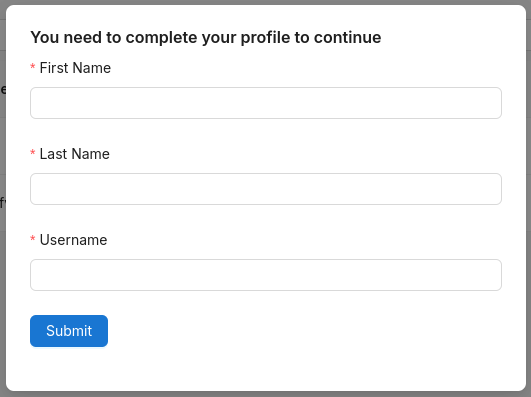
\includegraphics[scale=0.4]{images/fill-data-prompt.png}
    \caption{Prompt to fill in personal information.}
    \vspace{-1em} % Negative value to remove space
    \label{fig:prompt-fill-personal-information}
\end{figure}

% TODO: cite paper or something to show that this can happen?? im sure theres going to be
% smth
The \lstinline{image} field is used to store a URL to a user's profile picture. This field
can only be set if the user signed in with an OAuth 2.0, which supplied
the URL.
We don't accept custom URLs, as this allows for attackers to supply URLs to a server he
controls, which can be used to track user's browsers.
By only saving URLs provided directly by trusted OAuth 2.0 providers, we ensure that the
source of the image is reliable.

As stated before, we need Accounts, to store the sign-in methods of a user.
To recognize a user's account we need to store the name of the provider and the account's.
ID on the provider's platform.
Additionally, to link the account to a user, we store the user's ID in the account.
The schema for accounts is as follows:

\begin{lstlisting}[
  language=JavaScript,
  style=codestyle,
  caption={Schema for accounts.},
]
{
    id: string;
    type: "oauth";
    userId: string;
    provider: string;
    providerAccountId: string;
}
\end{lstlisting}

\subsection{Guest Users}

Users that aren't signed in can choose to try the MS out as a guest, this doesn't require
the user to input any personal information.
For users that choose to sign in as a guest, a new user is created and stored in the MS.
To achieve this, we use a modified version of the authenticated user schema described in
\ref{lst:authenticated-users-schema}, to only include the \lstinline{id} and the
\lstinline{isGuest} flag set to true.

\begin{lstlisting}[
  language=JavaScript,
  style=codestyle,
  caption={Schema for guest users.},
]
{
    isGuest: true;
    id: string;
} 
\end{lstlisting}

This option must be made available to users during the sign-in process. 
To accomplish this, NextAuth.js provides a built-in \lstinline{CredentialsProvider}, 
which enables the implementation of custom sign-in methods. 
We configured this provider to accept no credentials,
allowing users to sign in without supplying personal information.

\begin{lstlisting}[
  language=JavaScript,
  style=codestyle,
  caption={Custom sign-in method for guest users.},
]
import NextAuth from 'next-auth/next';

const authOptions = {
  providers: [
    ...
    CredentialsProvider({
      name: 'Continue as Guest',
      credentials: {},
      async authorize() {
        return addUser({ isGuest: true });
      },
    }),
  ],
}

const handler = NextAuth(authOptions)
\end{lstlisting}

After a user signs in as a guest, a JWT token is stored in his cookies.
Since there is no personal information stored, there is no way for the user to sign in to
his guest account from another device.
This also means, that if the cookies are deleted, the user will lose access to his guest account.

\subsection{Merge guest user data with an authenticated user's data}
\label{cha:ms-architecture:merge-guest-user-data}

When a guest user decides to sign in with personal information, we have to merge the data

\subsection{Development users}
\label{cha:ms-architecture:users:development-users}

\section{Assets}

- environmentId stored on each thing to improve querying
- talk about data normalization
- talk about breaking normalization for perfomance gains -> reference a paper or smth

\section{Environments}

- environments are entry in db
- memberships
- environment format entry
- verification (when envs are created by not signed in users)
- creation
- deletion - managing the env
- section for folders
- decide how to divide 

Environments are stored as an entry in the MS table


\subsection{Creation}
\subsection{Memberships}

\section{Roles}


